\documentclass[conference]{IEEEtran}
\IEEEoverridecommandlockouts

\usepackage{cite}
\usepackage{amsmath,amssymb,amsfonts}
\usepackage{algorithmic}
\usepackage{graphicx}
\usepackage{textcomp}
\usepackage{xcolor}
\usepackage{booktabs}
\usepackage{multirow}
\usepackage{url}
\usepackage{subcaption}
\usepackage{float}
\def\BibTeX{{\rm B\kern-.05em{\sc i\kern-.025em b}\kern-.08em
		T\kern-.1667em\lower.7ex\hbox{E}\kern-.125emX}}

\begin{document}
	
	\title{Autonomous Human Search System Using a Holybro S500 Drone With a Fixed Monocular Camera Based on Raspberry Pi 5}
	
	\author{\IEEEauthorblockN{Mahija Ibad Pradipta}
		\IEEEauthorblockA{\textit{Department of Computer Engineering} \\
			\textit{Institut Teknologi Sepuluh Nopember}\\
			Surabaya, Indonesia \\ mahijapradipta86@gmail.com}
		\and
		\IEEEauthorblockN{Dr. Arief Kurniawan, S.T., M.T.}
		\IEEEauthorblockA{\textit{Department of Computer Engineering} \\
			\textit{Institut Teknologi Sepuluh Nopember}\\
			Surabaya, Indonesia \\ arifku@ee.its.ac.id}
		\and
		\IEEEauthorblockN{Dr. Eko Mulyanto Yuniarno, S.T., M.T.}
		\IEEEauthorblockA{\textit{Department of Computer Engineering} \\
			\textit{Institut Teknologi Sepuluh Nopember}\\
			Surabaya, Indonesia \\ ekomulyanto@its.ac.id}
	}
	
	\maketitle
	
	\begin{abstract}
The advancement of Unmanned Aerial Vehicle (UAV) technology presents significant opportunities to accelerate Search and Rescue (SAR) operations in hard-to-reach disaster areas. This research designs and implements an autonomous system on a Holybro S500 drone for real-time human detection based on edge computing using a Raspberry Pi 5 and a monocular camera. The platform integrates a Pixhawk 6C flight controller, executing flight commands via MAVLink through the MAVSDK-Python library. Based on empirical evaluations, a fine-tuned YOLOv8n model in ONNX format at $320 \times 320$ pixel resolution was selected for its consistency in maintaining target bounding boxes during outdoor flight testing compared to pose-estimation variants. System software is built upon an asynchronous multi-threading architecture, supported by a stable power distribution system utilizing a 5A UBEC regulator to prevent system sags. Flight testing demonstrated continuous Scout Mission navigation through a state machine cycle consisting of scanning, approach, documentation, and displacement phases without requiring mid-mission landings. Furthermore, a multi-layered safety system mitigates sensor anomalies caused by barometric altitude drift during low-altitude maneuvers. The resulting prototype integrates visual perception, autonomous decision-making, and real-time telemetry streaming to support victim search missions.
\end{abstract}
	
	\begin{IEEEkeywords}
		Autonomous Drone, Edge Computing, MAVSDK-Python, Raspberry Pi 5, Search and Rescue, YOLOv8n
	\end{IEEEkeywords}
	
	\section{Introduction}
The continuous advancement of Unmanned Aerial Vehicle (UAV) technology provides critical capabilities for Search and Rescue (SAR) operations, especially in inaccessible disaster areas. UAVs improve mission success rates by expanding search coverage and providing real-time aerial data \cite{b1}. Rotary-wing drones, such as quadcopters, are advantageous for SAR due to their hovering capabilities and maneuverability \cite{b8}.

In Indonesia, which experiences high frequencies of natural disasters \cite{b3}, the adoption of drones for humanitarian operations remains limited by technological constraints in extreme conditions, lack of portable computing power, and the complexity of autonomous control \cite{b4}.

Conventional drone SAR operations often rely on manual control and raw video transmission to a Ground Control Station (GCS). This introduces latency, stuttering, and signal loss in post-disaster environments with unstable networks. To address these limitations, this research proposes an edge computing approach to process visual data directly on board the aircraft.

This study details the design of a fully autonomous drone integrating a Pixhawk 6C flight controller with a Raspberry Pi 5 companion computer. This enables local execution of the YOLOv8n object detection model without relying on GCS data links. The system navigates, detects humans, approaches, and documents targets autonomously.

The primary objectives are to develop a stable hardware and power architecture, evaluate YOLOv8n ONNX inference performance on a headless OS, and construct a Persistent Multi-Target Scouting finite state machine (FSM) utilizing MAVSDK-Python.

The scope is limited to a single Holybro S500 UAV. Edge computing relies on a single Raspberry Pi 5 (8GB) running a headless Linux OS to conserve resources. Local video recording is disabled to prevent I/O bottlenecks. Detection relies on a static monocular RGB camera identifying only the human class. Target duplicate exclusion is managed using GPS-based Haversine distance calculations.

\section{Related Work}
This research is supported by and built upon various comprehensive studies from previous experts relevant to the development of autonomous drones, power systems, and object detection systems for rescue missions.

\subsection{Autonomous Search and Rescue Drone architectures}
Elashaal et al. (2024) \cite{b5} developed an autonomous SAR drone using the Holybro S500, Pixhawk 2.4.8, and Raspberry Pi 4. The system utilized YOLOv4-tiny for real-time human detection, achieving a mAP of 96.44\% on top-view imagery. However, the architecture experienced high latency and low frame rates due to the computational limits of the Raspberry Pi 4. Field testing was restricted to open environments without vertical obstacles, lacking adaptive navigation logic for close-up target approaches. Furthermore, their power architecture relied heavily on generic step-down regulators, which are highly susceptible to voltage sagging when the flight controller and edge computer draw peak current simultaneously.

\subsection{Real-Time Human Detection and Navigation for SAR}
Jayalath and Munasinghe (2021) \cite{b6} integrated a TensorFlow Fast R-CNN detector with autonomous navigation on a Raspberry Pi 4 using the OkutamaAction dataset. The drone calculated GPS coordinates of victims based on geometric projection. Although achieving an 84.1\% accuracy, inference latency reached 8 seconds per frame. Such severe delays are entirely insufficient for dynamic real-world SAR missions requiring control feedback frequencies above 10 Hz. The detector was also highly vulnerable to varying sunlight conditions, often losing track of subjects when transitioning between shadows and direct sunlight.

\subsection{Target Detection, Tracking, and Avoidance System for UAVs}
Varatharasan et al. (2019) \cite{b7} optimized a low-cost hardware setup using a Raspberry Pi 3B+ and an Intel Movidius Neural Compute Stick 2 (NCS2). They utilized the MAVSDK API for OFFBOARD autonomous control, achieving system stability on low-power devices. However, the system required an external dedicated compute stick which adds mechanical payload weight and complexity to the electrical harness. Their depth estimation relied strictly on stadiametric rangefinding (estimating distance based on bounding box height), which is inherently prone to critical errors during sudden aircraft pitch or roll drifts where the geometric perspective is temporarily skewed.

\section{System Design and Architecture}
The system architecture was developed using an Engineering Design Process integrated with Systems Engineering principles. The design encompasses software processing pipelines, finite state machine navigation logic, computational power topology, and autonomous flight safety failsafes.

\subsection{Theoretical Background of Autonomous Systems and Edge Computing}
In UAV operations, edge computing shifts cognitive processing to the sensor source, eliminating bandwidth constraints and reducing decision-making latency \cite{b16}. This study utilizes YOLOv8n, a single-stage, anchor-free object detector, for its low latency on edge devices \cite{b11}. The YOLOv8 architecture replaces traditional C3 modules with C2f (Cross Stage Partial Bottleneck with two convolutions) blocks. This topological shift improves gradient flow and feature representation while maintaining a lightweight parameter count suitable for embedded Linux environments. Its structure comprises three primary segments: the CSPDarknet53 backbone for high-resolution feature extraction, the PANet (Path Aggregation Network) neck for multi-scale feature fusion across varying target distances, and a decoupled head that separates classification and bounding box regression tasks. Decoupling classification and regression accelerates Intersection over Union (IoU) loss convergence during training.

The pretrained YOLOv8n model was fine-tuned using the COCO2017 dataset, specifically filtered for the \textit{person} class to minimize inference overhead. To optimize execution performance, the PyTorch model was exported to the ONNX (Open Neural Network Exchange) format at a 320x320 input resolution. This quantization and serialization process maximizes parallel instruction efficiency on the Raspberry Pi 5's ARM Cortex-A76 cores, drastically reducing the thermal envelope compared to standard PyTorch inference. 

Communication between the companion computer and the Pixhawk 6C flight controller is handled via MAVLink, using MAVSDK-Python to translate logic scripts into asynchronous dynamic vector movement commands \cite{b12, b13}. The MAVLink protocol provides fault-tolerant serial transmission at a baud rate of 921600. It continuously transfers critical \texttt{HEARTBEAT} signals, \texttt{LOCAL\_POSITION\_NED} telemetry for Cartesian positioning, and \texttt{SET\_POSITION\_TARGET\_LOCAL\_NED} messages to dictate the drone's aerodynamic behavior. The overall system architecture is detailed in Figure \ref{fig:system_arch_full}.

\begin{figure*}[ht]
    \centering
    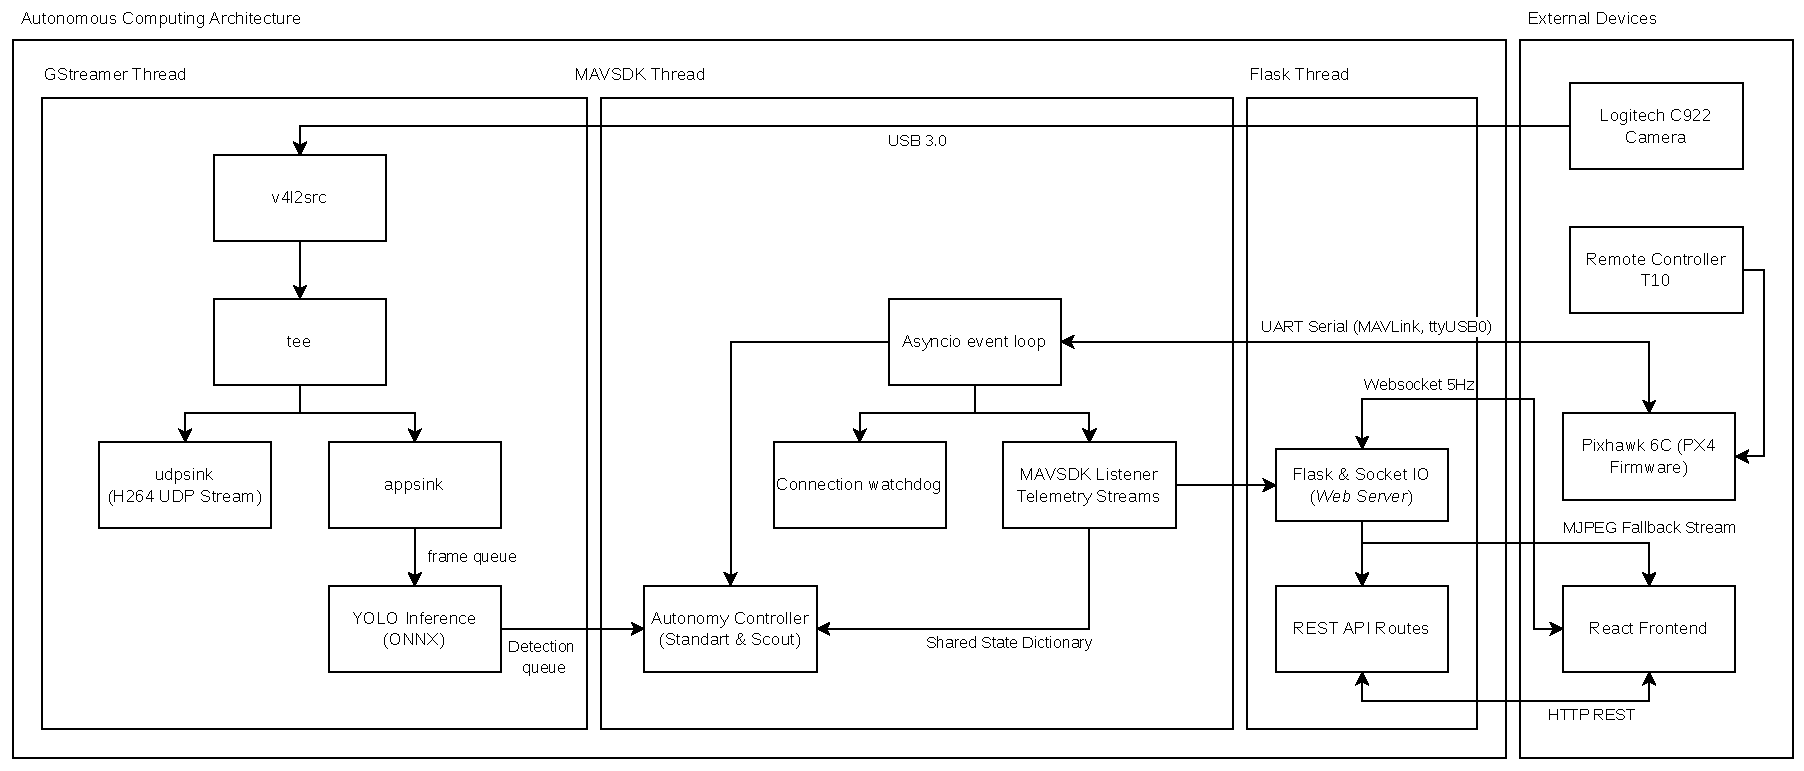
\includegraphics[width=0.85\linewidth]{figures/fig_system_arch.pdf}
    \caption{Overall System Architecture Topology showing interactions between the Pixhawk 6C (PX4 firmware), Raspberry Pi 5 companion computer, and Ground Control Station (GCS) operator interface.}
    \label{fig:system_arch_full}
\end{figure*}

\subsection{Design of the Autonomous Operation Cycle (Scout Mission)}
The system's autonomous behavior is governed by a Finite State Machine (FSM) termed the \textit{Scout Mission}. This architecture allows dynamic transitions based on environmental variables and computer vision outputs. The Scout Mission consists of four primary states (Figure \ref{fig:state_machine_fsm}):
\begin{itemize}
    \item SCAN State: The drone maintains a static hover while executing a slow yaw rotation at 20 degrees per second. To transition to the APPROACH state and eliminate visual clutter or transient noise, the detector must yield valid target detections across 3 consecutive frames (\texttt{SCOUT\_APPROACH\_CONFIRM\_FRAMES = 3}).
    \item APPROACH State: Upon locking onto a confirmed target, the drone initiates a forward approach using proportional error velocity setpoints. To trigger the DOCUMENT phase, the target must remain horizontally centered and within proximity criteria for 5 consecutive frames (\texttt{SCOUT\_DOCUMENT\_CONFIRM\_FRAMES = 5}) to ensure dynamic drone oscillations have fully settled. Furthermore, a safety timeout aborts pursuit and falls back to SCAN if target vision is lost for $>2.0$ s or if the approach duration exceeds $20.0$ s.
    \item DOCUMENT State: When documentation criteria are satisfied, the system records GPS coordinates and saves a full-resolution image.
    \item DISPLACING State: Instead of executing a mandatory Return-to-Launch (RTL), the drone performs a 2-meter lateral step displacement to exit the immediate discovery area and re-enters the SCAN state for continued observation.
\end{itemize}

\begin{figure}[ht]
    \centering
    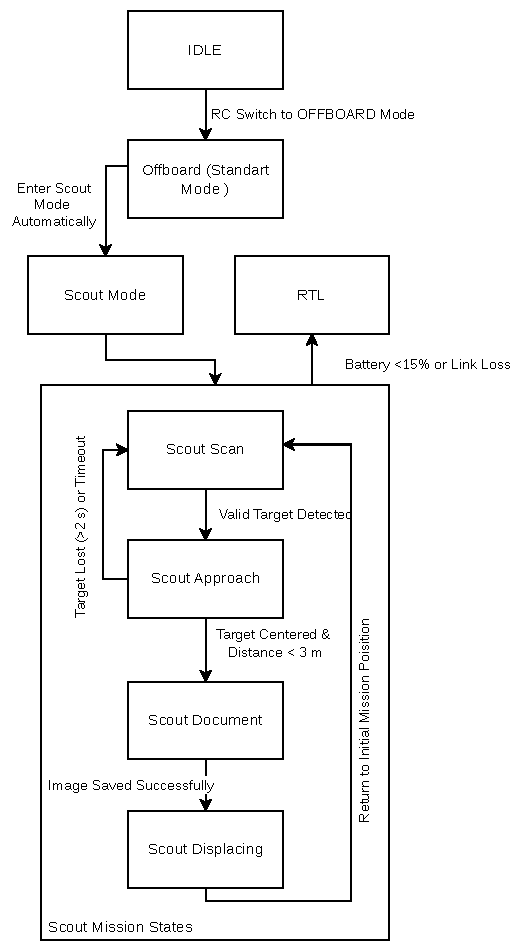
\includegraphics[width=0.9\linewidth]{figures/fig_state_machine.pdf}
    \caption{State Machine Diagram of the autonomous Scout Mission system, showing state transitions (SCAN, APPROACH, DOCUMENT, DISPLACING) and Target Lost Failback logic.}
    \label{fig:state_machine_fsm}
\end{figure}

This architecture enables Persistent Multi-Target Scouting, allowing the drone to search continuously until critical battery levels trigger RTL. To prevent duplicate documentation of the same target, a Duplicate Exclusion Memory algorithm is implemented using the Haversine geodesic distance formula:
\begin{equation}
a = \sin^2\left(\frac{\Delta\phi}{2}\right) + \cos\phi_1 \cdot \cos\phi_2 \cdot \sin^2\left(\frac{\Delta\lambda}{2}\right)
\end{equation}
\begin{equation}
c = 2 \cdot \text{atan2}\left(\sqrt{a}, \sqrt{1-a}\right)
\end{equation}
\begin{equation}
d = R \cdot c
\end{equation}
where $\phi_1$, $\phi_2$ are the latitudes of the two GPS points, $\Delta\phi = \phi_2 - \phi_1$ and $\Delta\lambda = \lambda_2 - \lambda_1$ are the latitude and longitude differences, $a$ is the spherical haversine value, $c$ is the angular distance in radians, $d$ is the geodesic surface distance in meters, and $R = 6,371,000$ m is Earth's mean radius. An absolute geospatial exclusion radius is enforced at 3.0 meters ($d \leq 3.0$ m). Detections falling within this radius of previously documented targets are bypassed, allowing persistent area coverage.

\subsection{Hardware and Electrical Topology}
The power system distributes energy from a single Tattu 4S Lithium Polymer (LiPo) battery (14.8V DC). Energy flows through a Holybro Power Module and Power Distribution Board (PDB) to the Electronic Speed Controllers (ESC) powering the propulsion motors.

For the Raspberry Pi 5, which demands high peak currents (up to 5A), standard power delivery methods such as GPIO-connected Mini UPS or basic step-down converters (e.g., XL4015E1) proved inadequate, leading to voltage sag, PMIC (Power Management Integrated Circuit) damage, or under-voltage throttling. The final robust design utilizes a 5A Universal Battery Elimination Circuit (UBEC). The UBEC connects in parallel to the main LiPo battery via an XT60 Y-splitter, providing a stable 5.1V DC supply via USB-C. This topology (Figure \ref{fig:electrical_design}) ensures reliable power delivery, preventing voltage drops during computationally intensive inference tasks and flight maneuvers.

\begin{figure}[ht]
    \centering
    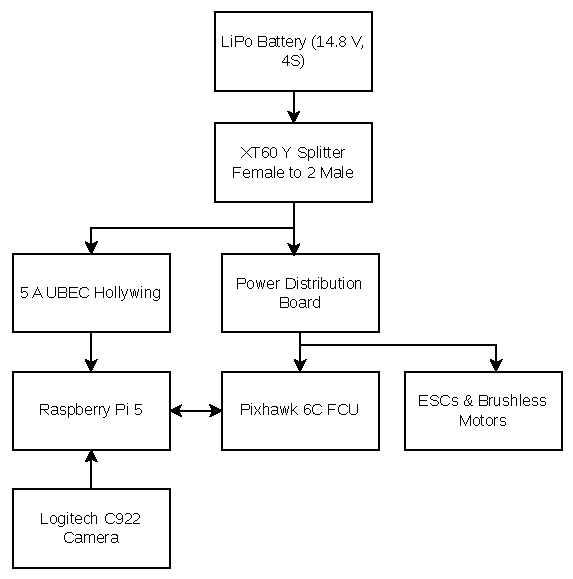
\includegraphics[width=0.95\linewidth]{figures/fig_electrical.pdf}
    \caption{Block diagram of the single battery (parallel) electrical load distribution architecture utilizing a 5A UBEC step-down module.}
    \label{fig:electrical_design}
\end{figure}

\subsection{Mechanical Component Integration}
The mechanical design emphasizes optimal Center of Gravity (CG) placement. Custom Fused Deposition Modeling (FDM) 3D-printed mounts, using Polylactic Acid (PLA), were fabricated for the components. This includes a tiered compartment for the LiPo battery, a ventilated housing for the Raspberry Pi 5, a UBEC protective case, and a vibration-dampened monopod for the static webcam at the lowest CG point. Figure \ref{fig:drone_assembly_real} illustrates the integrated hardware subsystems.

\begin{figure}[ht]
    \centering
    \begin{subfigure}[b]{0.57\linewidth}
        \centering
        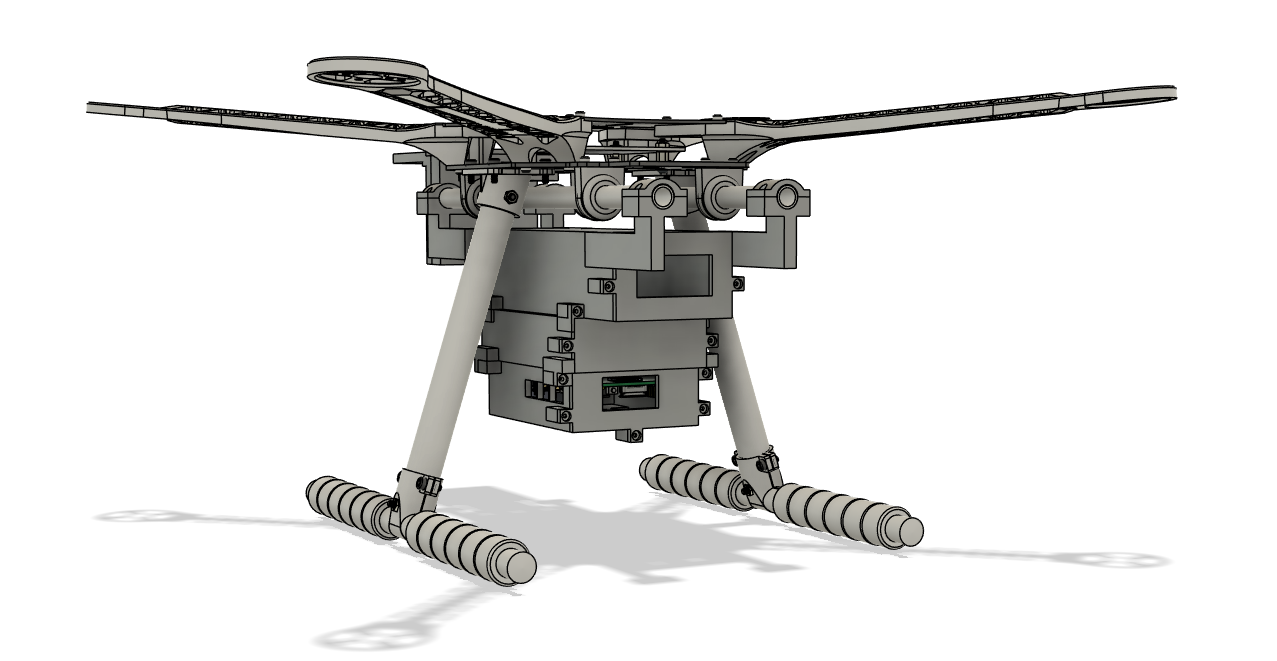
\includegraphics[width=\textwidth]{figures/fig_cad_assembly_bab3.png}
        \caption{Final CAD assembly}
        \label{fig:cad_assembly}
    \end{subfigure}
    \hfill
    \begin{subfigure}[b]{0.39\linewidth}
        \centering
        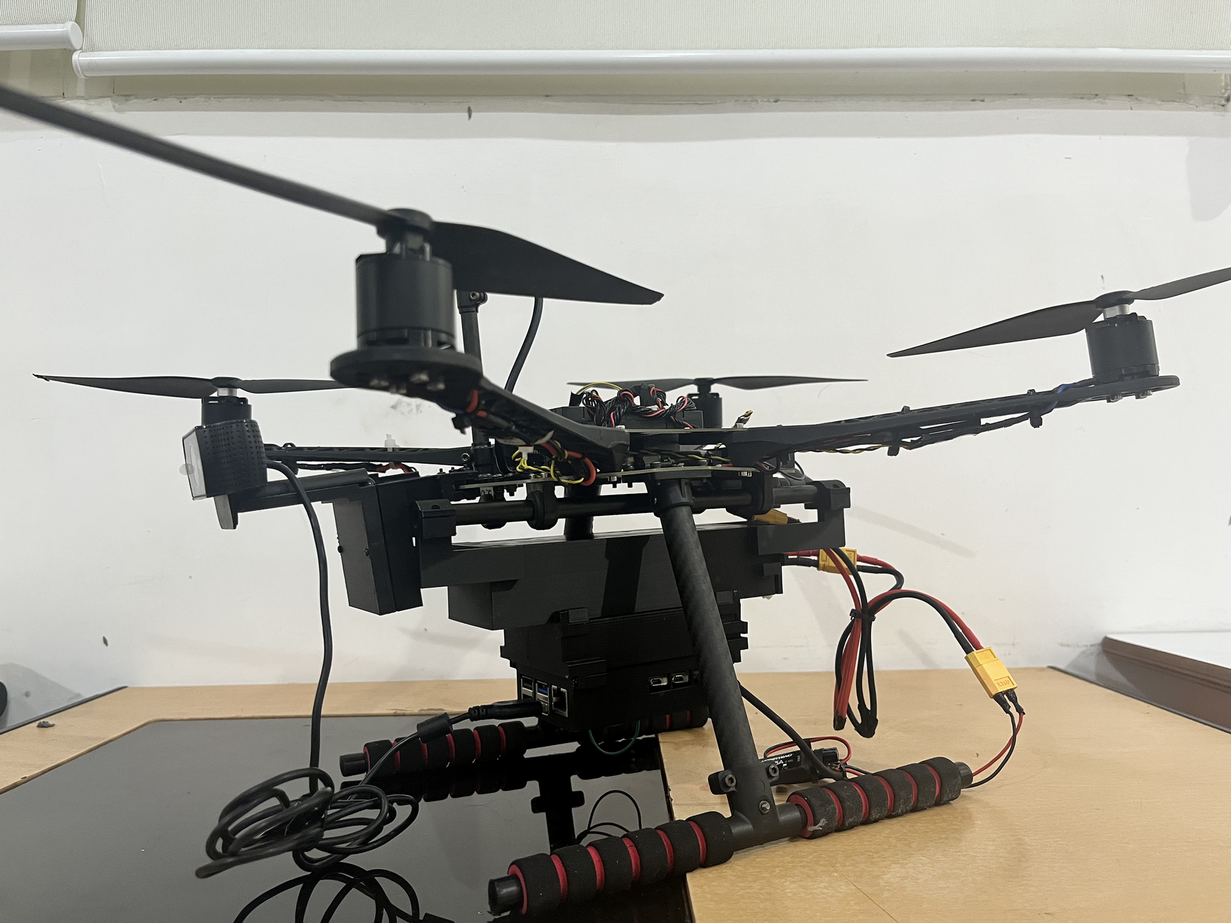
\includegraphics[width=\textwidth]{figures/fig_real_prototype_bab3.png}
        \caption{Realized prototype}
        \label{fig:real_prototype}
    \end{subfigure}
    \caption{Final UAV mechanical design and realized prototype.}
    \label{fig:drone_assembly_real}
\end{figure}

\subsection{Distributed Multithreading Edge Software Architecture}
The software architecture utilizes multi-threading to ensure that resource-intensive AI operations do not block the critical flight control loops. The Python \texttt{threading} module is employed to partition these tasks across the Raspberry Pi 5's quad-core CPU, decoupling asynchronous I/O and computer vision processing:
\begin{itemize}
    \item Main Execution Thread: Manages the Flask REST and SocketIO server for two-way WebSocket communication with the ground station.
    \item MAVSDK Telemetry Listener Thread: Operates asynchronously to manage flight telemetry and drive the FSM cycle at a strict 20 Hz loop.
    \item GStreamer Video Source Producer Thread: Captures frames via \texttt{v4l2src} and utilizes a tee-branch pipeline: one branch encodes H.264 video for low-latency UDP GCS transmission, while the second branch pushes raw RGB frames into a thread-safe leaky Frame Queue.
    \item YOLO Inference Consumer Thread: Dequeues frames, executes ONNX Runtime inference, and evaluates candidate target scores.
\end{itemize}
The complete data flow follows the Visual-to-Control Pipeline illustrated in Figure~\ref{fig:visual_control_pipeline}. Raw camera frames acquired via GStreamer are distributed by a tee branch into a thread-safe leaky Frame Queue. Frames are then evaluated by the ONNX Runtime engine, generating velocity vector setpoints transmitted via MAVSDK-Python to the Pixhawk 6C flight controller.

\begin{figure}[ht]
    \centering
    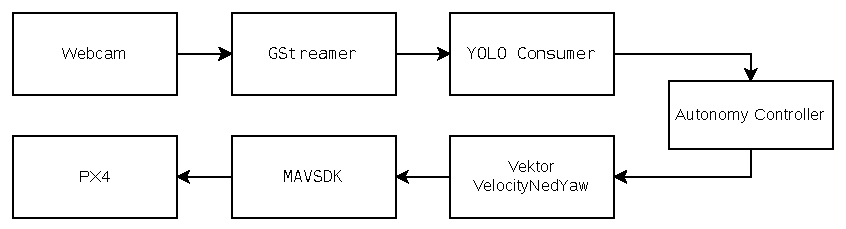
\includegraphics[width=0.98\linewidth]{figures/fig_visual_control_pipeline.pdf}
    \caption{Visual-to-Control Pipeline data flow mapping raw optical inputs to autonomous flight velocity setpoints.}
    \label{fig:visual_control_pipeline}
\end{figure}

\subsection{Proportional Navigation Control Loop and Target Lock Hysteresis}
To translate conceptual logic into flight maneuvers, a proportional navigation algorithm was implemented. The system periodically calculates the pixel alignment error between the target's bounding box center and the camera frame's geometric center. Because raw bounding box coordinates contain noise from wind and drone vibrations, an Adaptive Exponential Moving Average (EMA) filter is applied:
\begin{equation}
S_t = \alpha \cdot x_t + (1 - \alpha) \cdot S_{t-1}
\end{equation}
The smoothing factor $\alpha$ is set adaptively: $\alpha = 0.20$ when the target is distant (Bounding Box Area ratio $\leq 0.20$), increasing to $\alpha = 0.30$ as the target approaches (Bounding Box Area ratio $> 0.20$).

To evaluate candidate target detections and prevent erratic target switching (\textit{target ping-ponging}) when multiple human subjects appear in the camera's FOV, a linear weighted scoring formula is evaluated:
\begin{equation}
\text{Score} = 0.45 \cdot A_{\text{box}} + 0.25 \cdot C_{\text{score}} + 0.20 \cdot D_{\text{center}} + 0.10 \cdot H_{\text{track}}
\end{equation}
where $A_{\text{box}}$ is the normalized bounding box area ratio (proximity metric), $C_{\text{score}}$ is the YOLO confidence score, $D_{\text{center}} = 1 - \frac{|err_x|}{w_{\text{frame}}/2}$ is the horizontal centering metric, and $H_{\text{track}}$ is the spatial tracking history weight. Furthermore, a target lock hysteresis threshold requires any newly detected target score to exceed the currently locked target score by at least 35\% ($\Delta \text{Score} \geq 0.35$) before switching focus.

For lateral alignment, the yaw rate $\omega_z$ (deg/s) is defined linearly based on the horizontal pixel offset error ($err_x$) and gain $K_p$:
\begin{equation}
\omega_z = K_p \cdot err_x 
\end{equation}
Simultaneously, the forward approach velocity $v_x$ (m/s) is regulated by evaluating $A_{\text{box}}$ against optimal documentation threshold $A_{\text{opt}}$ with damping coefficient $\gamma$:
\begin{equation}
v_x = \gamma \cdot \left( A_{opt} - A_{box} \right)
\end{equation}
These mathematical variables combine to output velocity setpoints via MAVSDK-Python's \texttt{VelocityNedYaw} method operating in OFFBOARD flight mode.

\section{Implementation}

\subsection{Three-Layer Failsafe Safety Architecture}
To mitigate barometric altitude drift common in tropical field environments, a three-layer failsafe safety system is integrated directly into the autonomous flight core:
\begin{enumerate}
    \item Altitude Floor Clamping: The minimum safe altitude is strictly constrained to 1.2 meters, preventing any autonomous command from forcing the drone to descend into the ground or jungle canopy.
    \item Runtime Setpoint Rejection: At a 20 Hz loop rate, if the navigation algorithm outputs a target descent velocity (\texttt{target\_alt}) that breaches the 1.2-meter limit, the command is instantly rejected and replaced with a zero-velocity vector, forcing the drone into a static hover.
    \item Pre-RTL Safety Climb: When PX4 detects a critical low battery threshold, it defaults to a straight Return-to-Launch trajectory. However, the companion computer intercepts this event and commands an immediate Pre-RTL Safety Climb vector (-0.8 m/s vertical velocity for 3.0 seconds). This vertical climb gains obstacle clearance before PX4 assumes final RTL control.
\end{enumerate}

Additionally, an overarching heartbeat monitor ensures that if the MAVSDK-Python \texttt{HEARTBEAT} transmission fails to arrive at the Pixhawk within a 500 ms timeout threshold—due to a Raspberry Pi software crash or serial cable disconnection—the Pixhawk will autonomously drop out of OFFBOARD mode and trigger a fallback HOLD or RTL state. This ensures the vehicle is never left flying blindly without algorithmic supervision.

\subsection{GCS Telemetry Pipeline and Operational Interface}
The Ground Control Station (GCS) interface operates via the Telemetry-to-Frontend Pipeline illustrated in Figure~\ref{fig:telemetry_pipeline}. High-frequency MAVLink telemetry is continuously captured from the Pixhawk 6C by the MAVSDK-Python listener at 20 Hz, cached in shared state memory, formatted by the Flask backend, and broadcast via SocketIO at 5 Hz to update the React 19 GCS operator HUD overlay. A Skydroid T10 remote controller provides a manual hardware override, immediately terminating OFFBOARD mode upon switch activation.

\begin{figure}[ht]
    \centering
    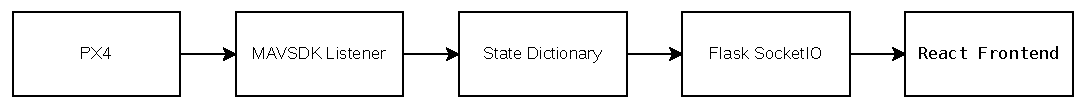
\includegraphics[width=0.98\linewidth]{figures/fig_telemetry_pipeline.pdf}
    \caption{Telemetry-to-Frontend Pipeline data flow mapping Pixhawk 6C sensor metrics to the React GCS dashboard.}
    \label{fig:telemetry_pipeline}
\end{figure}

\section{Experimental Results}
The system was evaluated through empirical testing across 5 in-flight testing sessions conducted at UNY Field. The flight test matrix recorded 38 total approach triggers, 30 successful target documentations, and 8 target loss instances caused by rapid out-of-FOV movements. Tests assessed power stability, algorithm accuracy, end-to-end latency, and navigation reliability.

\subsection{System Power Integrity and OS Optimization}
Testing the power architecture on the Raspberry Pi 5 showed that conventional Mini UPS modules or standard buck converters (e.g., XL4015E1) failed under peak computational loads. These failures caused PMIC damage or \textit{under-voltage} warnings that triggered system reboots. The final integration of a 5A UBEC directly connected to the main LiPo battery successfully provided a stable 5.1V DC supply, eliminating \textit{brownout} incidents even during peak inference loads.

Additionally, executing the system on a headless Linux OS (without a GUI) reduced idle RAM consumption from $\sim$1,200 MB to $\sim$420 MB. This optimization prevented frame dropping and latency spikes, enabling a stable processing pipeline.

\subsection{Detection Algorithm Architecture Evaluation}
An empirical evaluation was conducted comparing the baseline YOLOv8n model against its pose-estimation variant (YOLOv8n-pose). While the pose model identified skeletal keypoints, it exhibited bounding box flickering under varying outdoor illumination and motion blur during dynamic maneuvers. Consequently, the baseline YOLOv8n detector was selected for its robustness and consistent target accuracy during flight.

Further optimization focused on determining the optimal ONNX tensor input resolution. The computational benchmarking on the Raspberry Pi 5 measured the impact of three different tensor dimensions on the ONNX Runtime engine. As detailed in Table \ref{tab:model_comparison}, a 640x640 resolution resulted in an unacceptable latency of 171.22 ms (5.84 FPS), posing a severe risk to the real-time closed-loop control architecture. Conversely, a 256x256 resolution yielded 35.54 FPS but suffered from significant precision loss at distances exceeding 10 meters. Ultimately, the 320x320 resolution provided an optimal balance, reducing inference latency to 42.17 ms ($\sim$23.72 FPS) while maintaining sufficient accuracy for target detection.

\begin{table}[ht]
    \centering
    \caption{Benchmarking of YOLOv8n ONNX Input Resolutions on Raspberry Pi 5}
    \label{tab:model_comparison}
    \setlength{\tabcolsep}{4pt}
    \begin{tabular}{@{}ccccc@{}}
        \toprule
        \textbf{Model Variant} & \textbf{Input Size} & \textbf{Output Tensor} & \textbf{Avg FPS} & \textbf{Latency (ms)} \\
        \midrule
        256n & 256x256 px & [1, 84, 1344] & $\sim$ 35.54 & $\sim$ 28.13 \\
        \textbf{320n} & \textbf{320x320 px} & \textbf{[1, 84, 2100]} & \textbf{$\sim$ 23.72} & \textbf{$\sim$ 42.17} \\
        640n & 640x640 px & [1, 84, 8400] & $\sim$ 5.84  & $\sim$ 171.22 \\
        \bottomrule
    \end{tabular}
\end{table}

\subsection{YOLOv8n Transfer Learning and Fine-Tuning}
The selected YOLOv8n model was fine-tuned over 50 epochs using a filtered COCO2017 dataset containing 123,287 images limited strictly to the \textit{person} class. The training achieved convergence at the 40th epoch (Figure \ref{fig:training_loss_curves}). Validation metrics (Table \ref{tab:training_metrics_akhir}) confirm high performance: a Precision of 0.809, Recall of 0.646, and mAP@50 of 0.757. The peak F1-Score of 0.72 at a confidence threshold of 0.224 ensured reliable detection capability in the field.

\begin{figure}[ht]
    \centering
    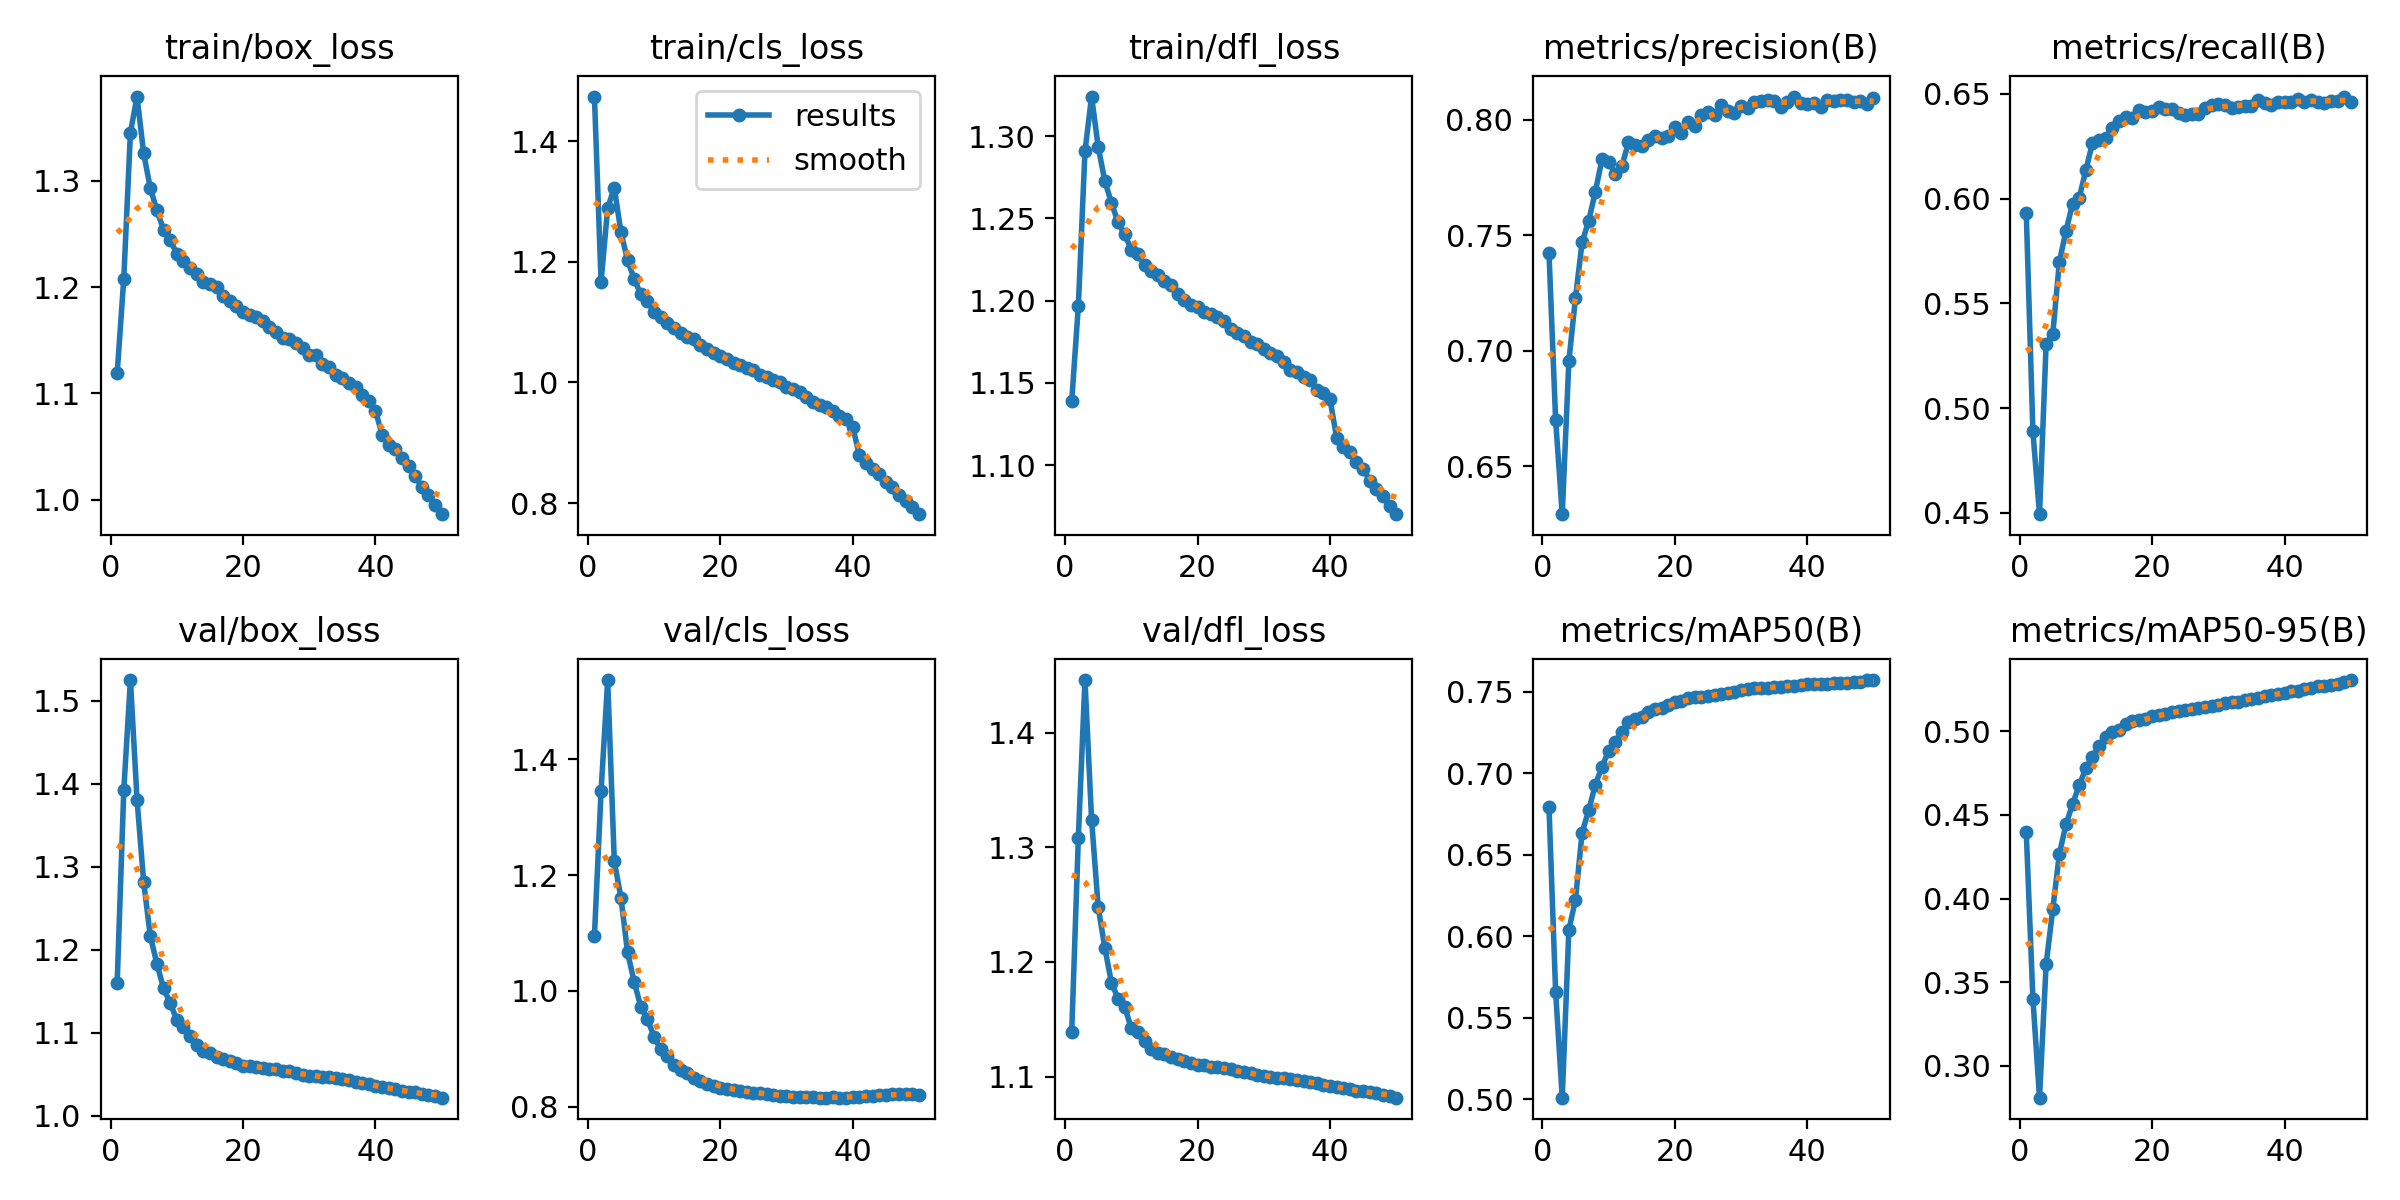
\includegraphics[width=0.85\linewidth]{figures/fig_training_results.png}
    \caption{Training and validation metric progression for the fine-tuned YOLOv8n model over 50 epochs.}
    \label{fig:training_loss_curves}
\end{figure}

\begin{table}[ht]
    \centering
    \caption{Evaluation Metrics for the Fine-Tuned YOLOv8n Model}
    \label{tab:training_metrics_akhir}
    \begin{tabular}{@{}p{5.5cm}r@{}}
        \toprule
        \textbf{Metric} & \textbf{Value} \\
        \midrule
        Precision & 0.809 \\
        Recall & 0.646 \\
        mAP@50 & 0.757 \\
        mAP@50-95 & 0.531 \\
        Peak F1-Score & 0.72 at Threshold 0.224 \\
        \bottomrule
    \end{tabular}
\end{table}

\subsection{Autonomous Flight Testing: FSM Scout Mission}
The Persistent Multi-Target Scouting FSM was validated across 38 approaching maneuver triggers during flight. The transition from SCAN to APPROACH operated flawlessly, recording a 100\% success rate. Furthermore, the drone successfully completed the DOCUMENT phase 30 times. Only 8 instances resulted in tracking failures, primarily due to targets moving rapidly outside the camera's narrow Field of View (FOV) during the APPROACH phase. In these cases, the autonomy safely executed a failback loop, immediately returning to the SCAN state without system failure. The FSM execution sequence is visualized in Figure \ref{fig:fsm_in_flight}.

\begin{figure}[ht]
    \centering
    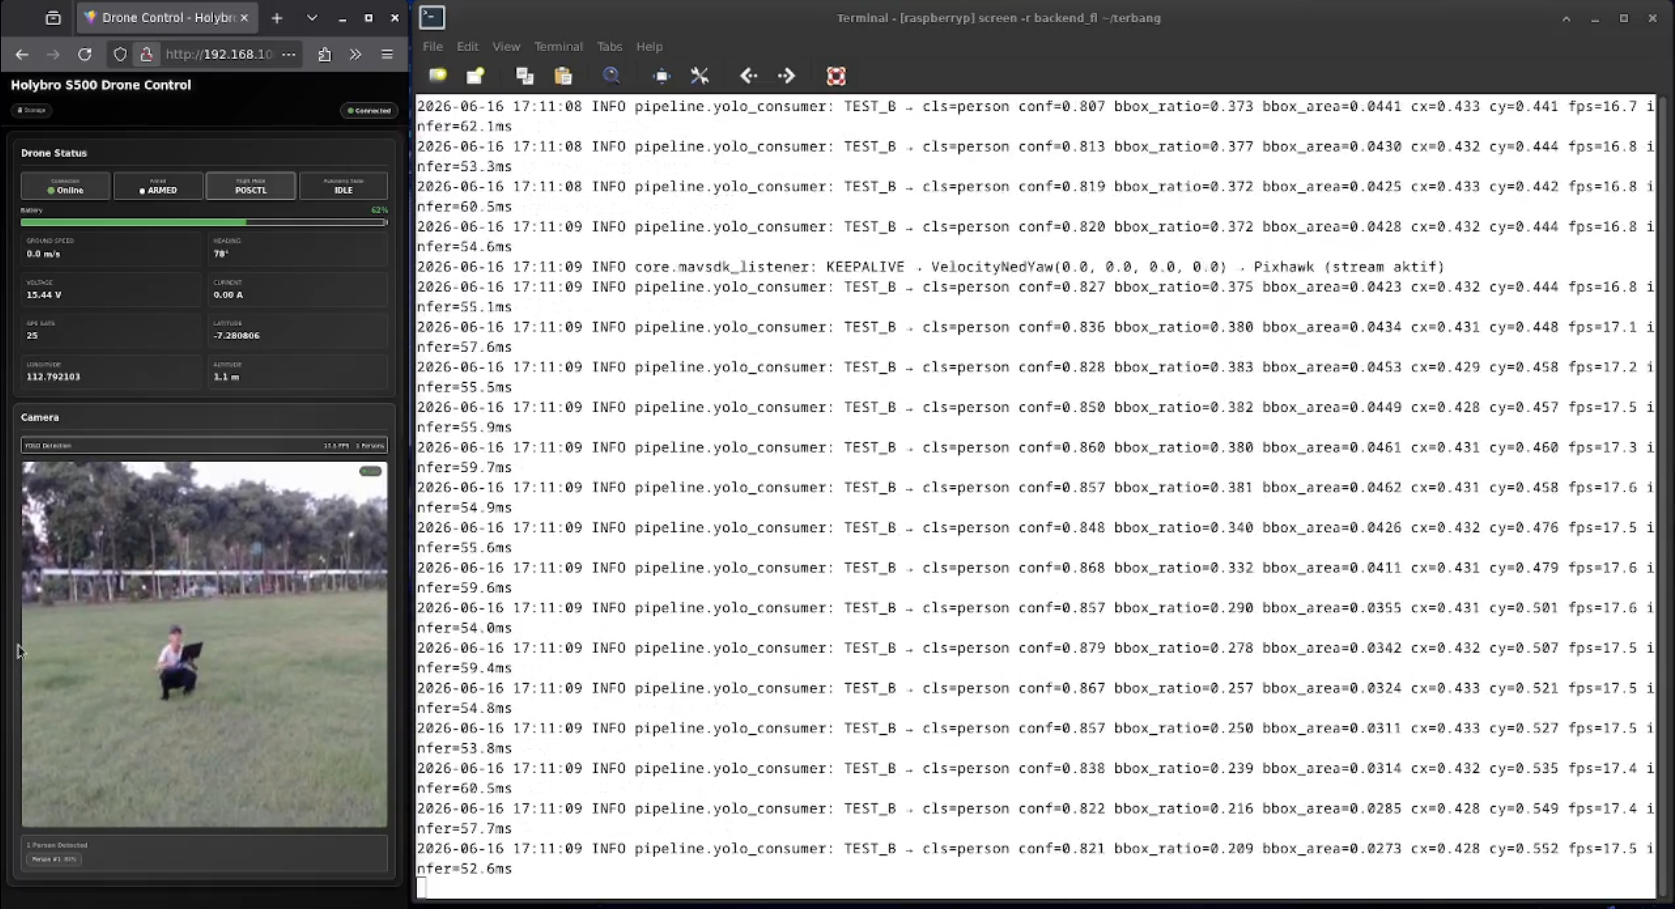
\includegraphics[width=0.85\linewidth]{figures/fig_fsm_berjalan.png}
    \caption{In-flight execution of the FSM Scout Mission showing active target detection during the APPROACH state.}
    \label{fig:fsm_in_flight}
\end{figure}



\subsection{In-Flight Visual Catch Distance Accuracy Test}
The endurance and tracking performance of the object detection algorithm were evaluated during stable hovering conditions at altitudes between 1 and 2 meters (AGL --- Above Ground Level). A test subject moved linearly away from the drone, increasing distance from 5 to 20 meters. Detection accuracy and bounding box stability were measured against the distance threshold. At ranges $\leq 15$ meters, the system maintained a 100\% detection success rate with consistent Bounding Box Area ratios. However, as the distance approached 20 meters, the target resolution on the 320x320 input grid became insufficient, resulting in increased tracking uncertainty and detection failures. The detection rate dropped to 45.5\% at the 20-meter mark, identifying this distance as the functional limit of the current optical configuration.

\begin{figure}[ht]
    \centering
    \begin{subfigure}[b]{0.45\linewidth}
        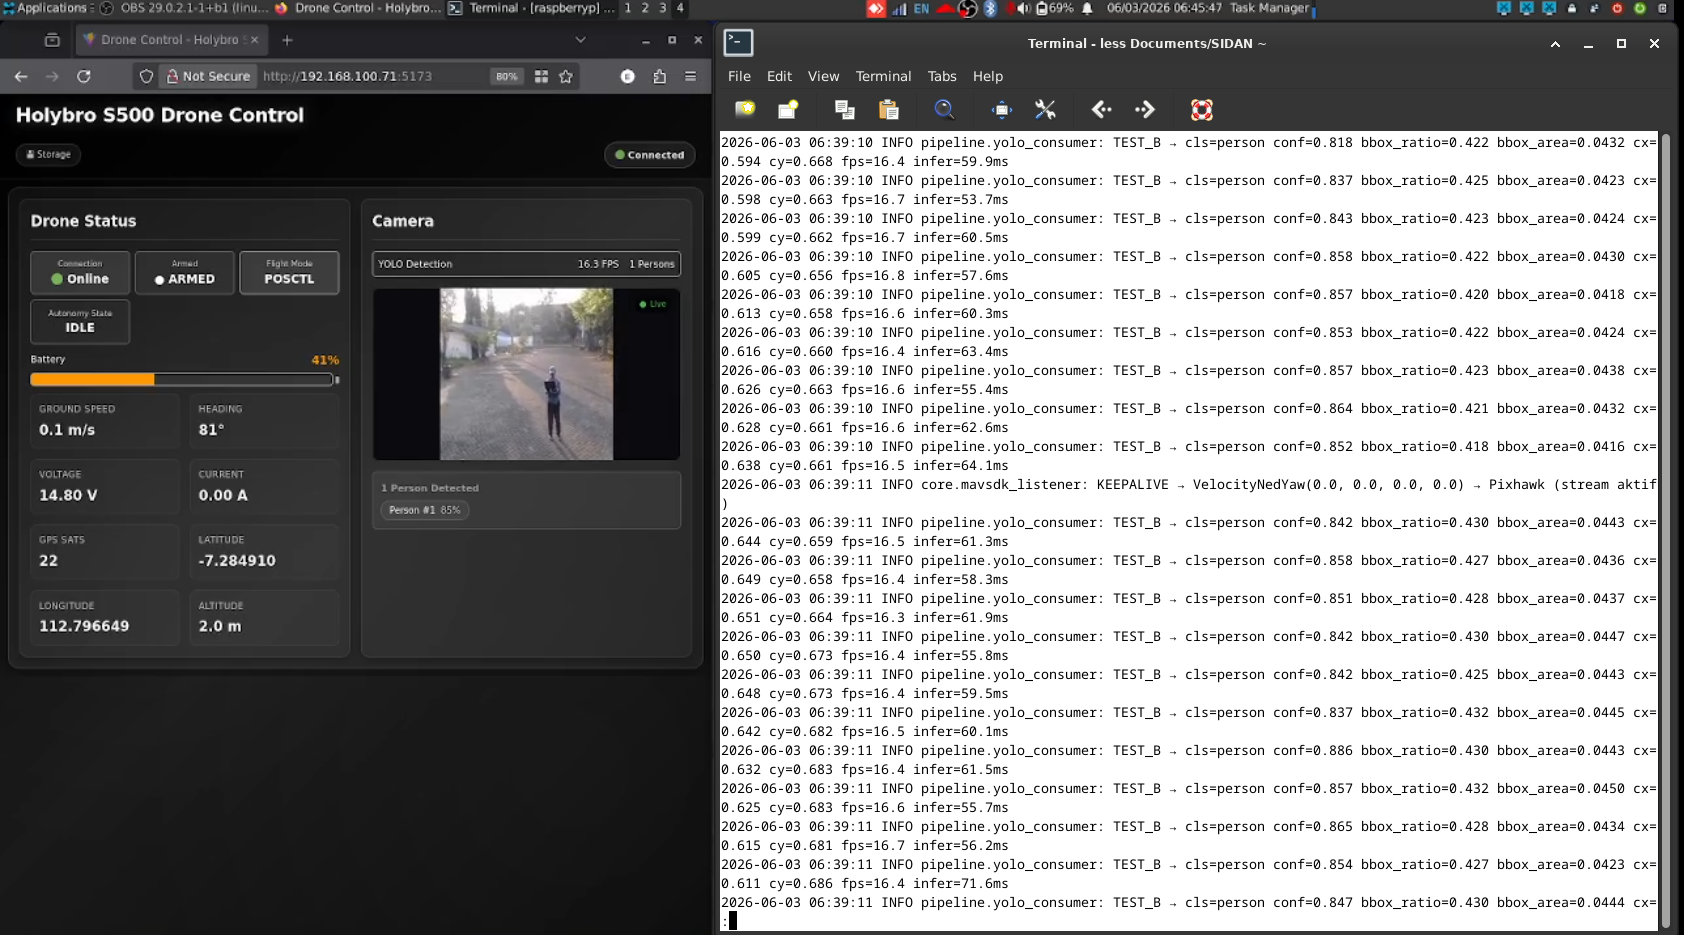
\includegraphics[width=\textwidth]{figures/fig_deteksi5m.png}
        \caption{Target detection at 5 m.}
    \end{subfigure}
    \hfill
    \begin{subfigure}[b]{0.45\linewidth}
        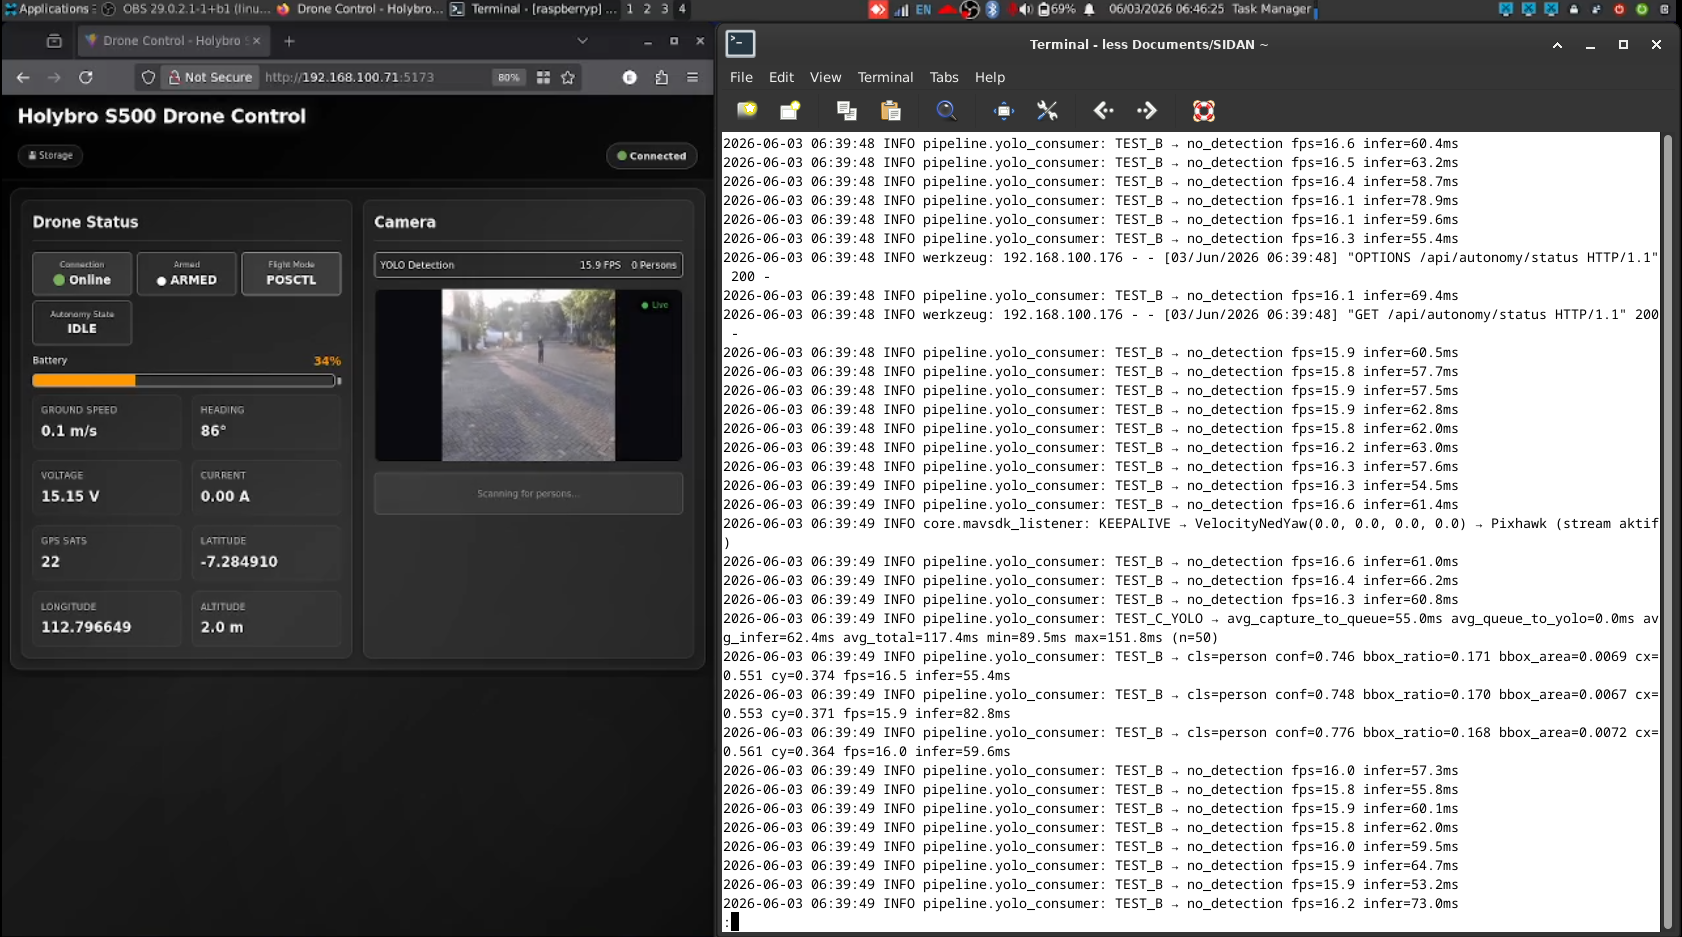
\includegraphics[width=\textwidth]{figures/fig_deteksi20m.png}
        \caption{Target detection at 20 m.}
    \end{subfigure}
    \caption{In-flight visual target detection performance at 5 m and 20 m operating distances.}
    \label{fig:in_flight_detection}
\end{figure}

\subsection{End-to-End Latency and Navigation Accuracy}
Latency tests across 2,096 samples over five flight sessions measured the total time from frame capture to the delivery of a velocity setpoint to the Pixhawk. The overall average end-to-end latency was 188.04 ms. The median (P50) latency was 164.65 ms, the 90th percentile (P90) was 192.30 ms, and the 95th percentile (P95) was 208.27 ms. Majority of processing cycles remain below 210 ms, meeting the requirements for real-time mission execution without destabilizing the drone. The detailed breakdown of the pipeline stages contributing to the total end-to-end latency is presented in Table \ref{tab:latency_breakdown}.

\begin{table}[ht]
    \centering
    \caption{End-to-End Pipeline Latency Breakdown (2,096 samples)}
    \label{tab:latency_breakdown}
    \setlength{\tabcolsep}{3pt}
    \begin{tabular}{@{}p{3.0cm}cccc@{}}
        \toprule
        \textbf{Pipeline Stage} & \textbf{Avg (ms)} & \textbf{Min (ms)} & \textbf{Max (ms)} & \textbf{Std Dev} \\
        \midrule
        Capture $\rightarrow$ Frame Queue & 41.87 & 0.5 & 57.4 & 21.45 \\
        Frame Queue $\rightarrow$ YOLO Start & 0.00 & 0.0 & 0.0 & 0.00 \\
        YOLO Inference (ONNX) & 59.08 & 49.9 & 76.8 & 4.42 \\
        Detection $\rightarrow$ Cmd Generation & 73.34 & 1.2 & 1380.1 & 164.71 \\
        \midrule
        \textbf{Total End-to-End} & \textbf{188.04} & \textbf{53.0} & \textbf{1602.2} & \textbf{185.10} \\
        \bottomrule
    \end{tabular}
\end{table}

Navigation accuracy was assessed via the horizontal alignment error during 30 documentation phases. The system achieved an average Bounding Box Area ratio of 0.389 and an average horizontal alignment error (\texttt{err\_x}) of 0.049 at the moment of documentation trigger. A 2.0-meter lateral displacement maneuver across 29 trials demonstrated minimal deviation, averaging 4.52\% error from the GPS destination, confirming precise setpoint synchronization between the Pixhawk EKF2 (Extended Kalman Filter 2) estimator and the companion computer.

\subsection{Failsafe Safety and Persistent Scouting}
\label{sec:results_failsafe}
The three-layer failsafe architecture effectively neutralized barometric altitude drift anomalies. During battery depletion tests (Battery RTL triggered at 13--14\% capacity), the drone successfully executed the Pre-RTL Safety Climb maneuver, achieving actual altitude gains ranging from 0.46 to 2.27 meters before initiating the horizontal RTL maneuver (Figure \ref{fig:battery_rtl}). The manual RC Override switch successfully terminated the autonomy script in all test cases.

\begin{figure}[h]
    \centering
    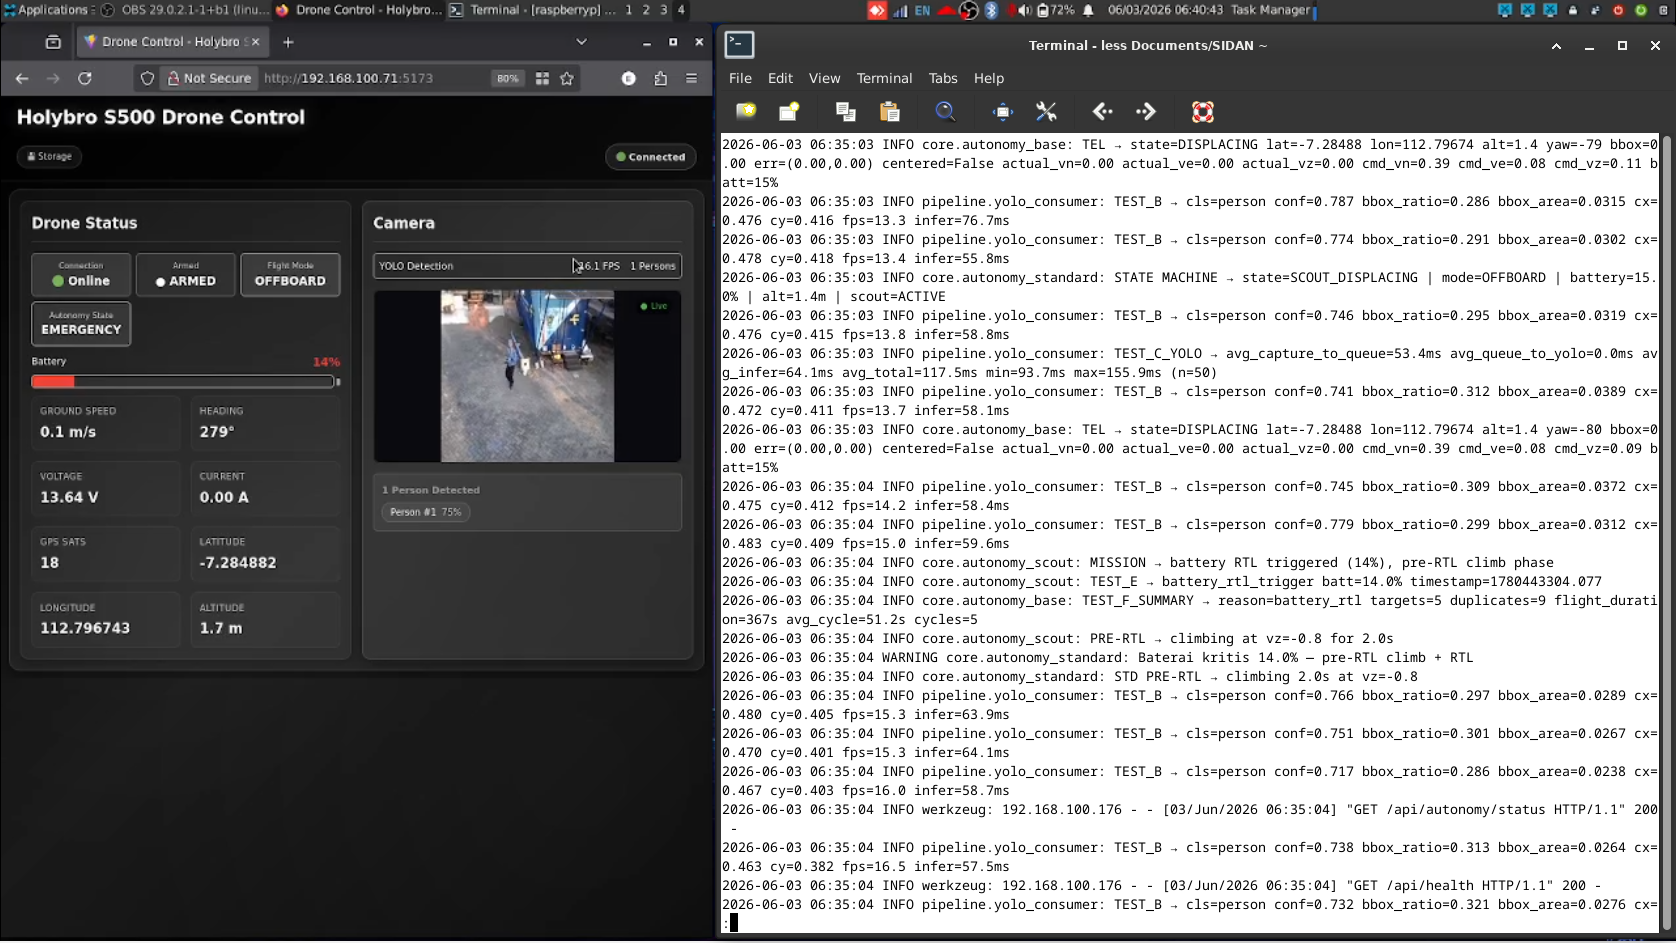
\includegraphics[width=0.8\linewidth]{figures/fig_battery_rtl.png}
    \caption{Flight log recording Battery RTL activation and execution of the Pre-RTL Safety Climb maneuver.}
    \label{fig:battery_rtl}
\end{figure}

The Persistent Scouting logic documented 11 distinct targets across five flight sessions. Utilizing the Haversine formula with a 3-meter exclusion radius, the system successfully bypassed 19 duplicate detections without triggering RTL, proving the drone's capability to continue area observation efficiently. The average tracking cycle duration was approximately 51--57 seconds per subject. During these intensive operations, the Raspberry Pi 5 maintained an average CPU utilization of 144.06\% (multi-core) with a peak of 177\%, and average RAM usage of approximately 600 MB (reducing idle footprint from $\sim$1,200 MB down to $\sim$420 MB via the headless Linux OS). Zero incidences of thermal throttling were observed, validating the headless OS and passive cooling design. Representative documented targets from these scouting sessions are shown in Figure~\ref{fig:persistent_scouting_proof}, and the corresponding GCS operator monitoring dashboard is shown in Figure~\ref{fig:dashboard_interface}.

\begin{figure}[ht]
    \centering
    \begin{subfigure}[b]{0.45\linewidth}
        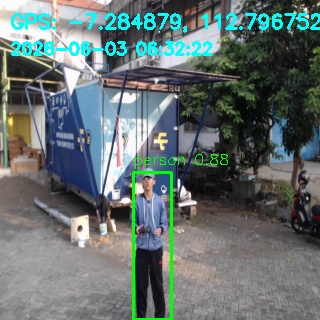
\includegraphics[width=\textwidth]{figures/fig_scout_morning.jpg}
        \caption{Target documented under morning light.}
    \end{subfigure}
    \hfill
    \begin{subfigure}[b]{0.45\linewidth}
        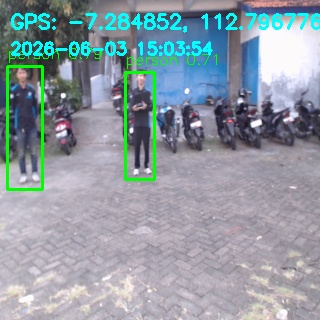
\includegraphics[width=\textwidth]{figures/fig_scout_day.jpg}
        \caption{Target documented under daytime light.}
    \end{subfigure}
    \vskip\baselineskip
    \begin{subfigure}[b]{0.45\linewidth}
        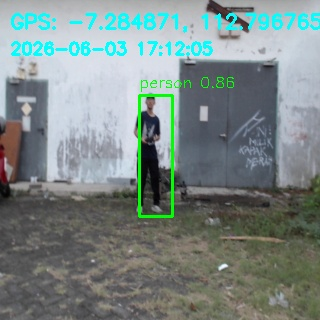
\includegraphics[width=\textwidth]{figures/fig_scout_dusk.jpg}
        \caption{Target documented under dusk light.}
    \end{subfigure}
    \hfill
    \begin{subfigure}[b]{0.45\linewidth}
        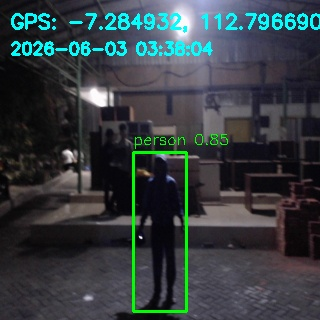
\includegraphics[width=\textwidth]{figures/fig_scout_night.jpg}
        \caption{Target documented under night lighting.}
    \end{subfigure}
    \caption{Target documentation outputs captured during Persistent Multi-Target Scouting missions across varying field lighting conditions.}
    \label{fig:persistent_scouting_proof}
\end{figure}

\begin{figure}[ht]
    \centering
    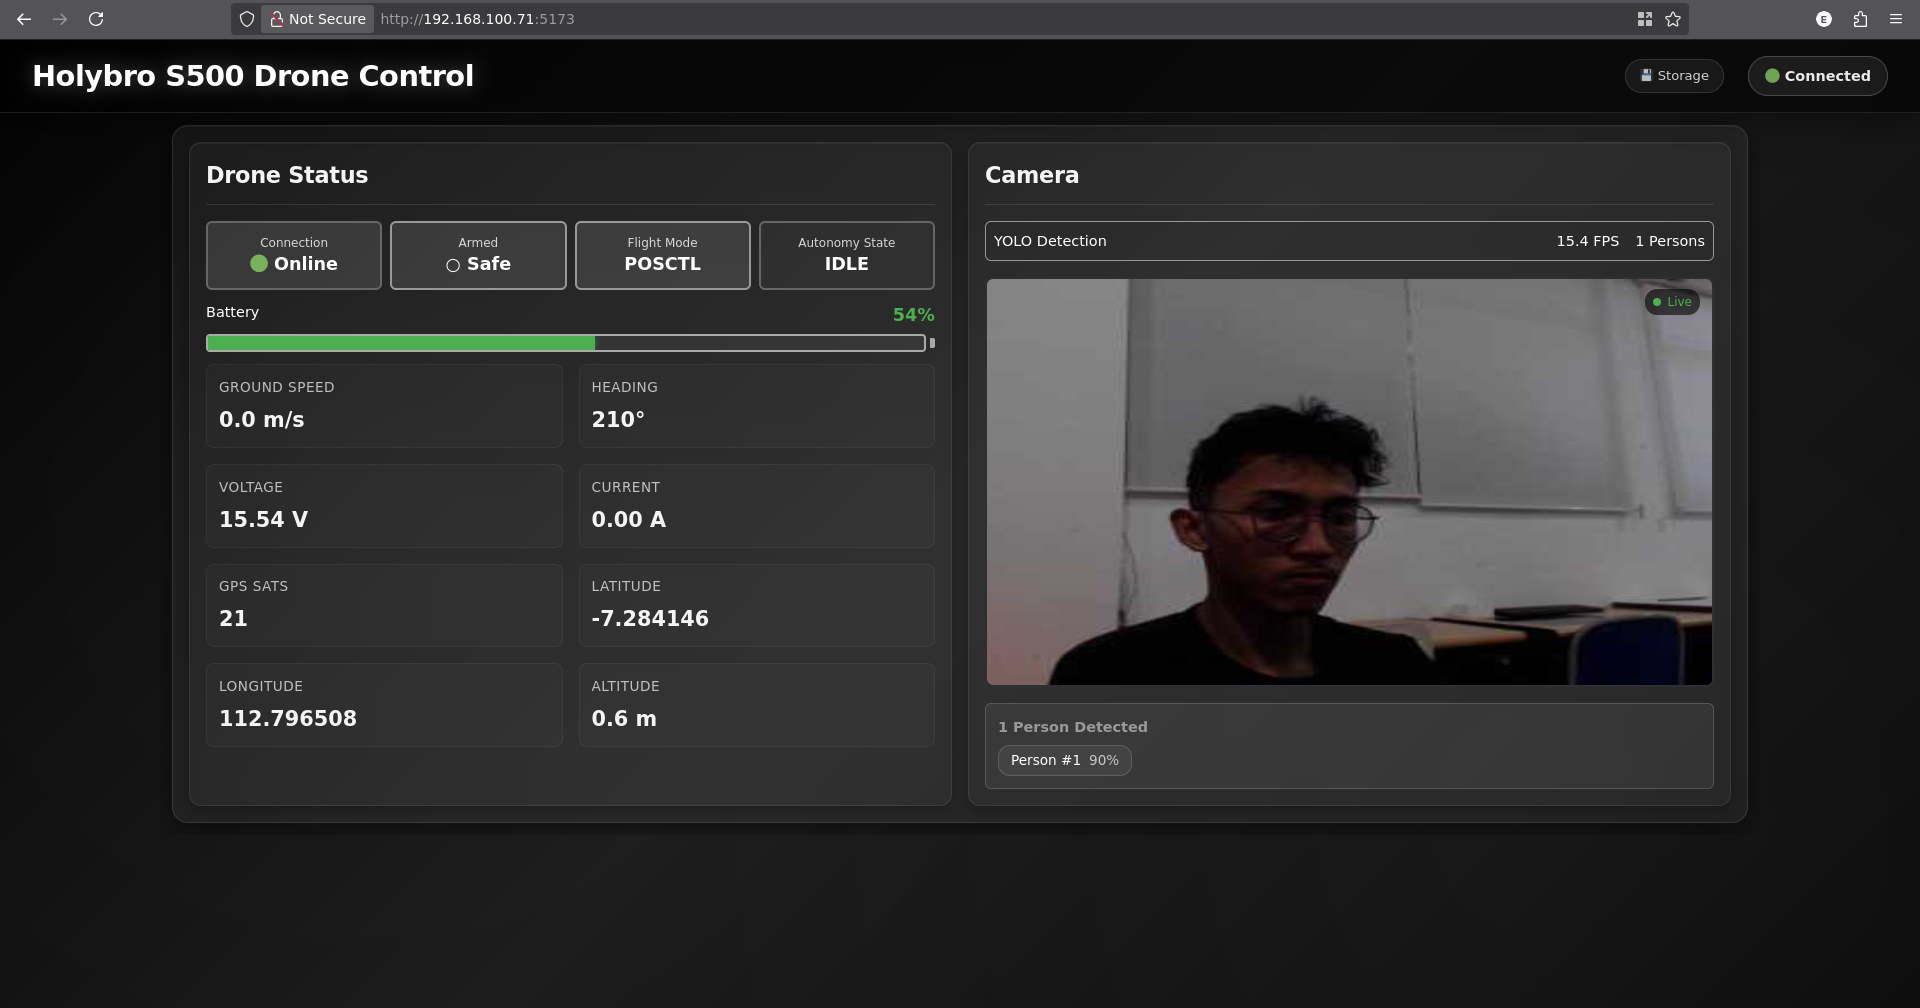
\includegraphics[width=0.95\linewidth]{figures/fig_dashboard.png}
    \caption{Real-time Ground Control Station (GCS) dashboard displaying flight telemetry, Scout Mission status, and system monitoring information.}
    \label{fig:dashboard_interface}
\end{figure}

\section{Discussion}
While the developed system demonstrated reliable autonomous SAR capabilities under the tested conditions, several critical hardware and software trade-offs must be acknowledged:
\begin{itemize}
    \item \textbf{Model Resolution Trade-offs}: Scaling down the YOLOv8n tensor to 320x320 pixels significantly improved inference latency, achieving approximately 23 FPS on edge hardware. Detection rates remained stable at 100\% up to 15 meters, but dropped to 45.5\% at 20 meters as the Bounding Box Area on the 320x320 input grid became insufficient. This forces the drone to conduct scouting missions at closer proximities.
    \item \textbf{Model Architecture Constraints}: The baseline YOLOv8n bounding box detector was chosen over YOLOv8n-pose due to lower computational overhead and greater resistance to motion blur. While skeletal keypoint data could theoretically improve posture analysis, the pose model proved unstable under varying outdoor illumination and camera perspective shifts during dynamic drone maneuvers, causing erratic navigation feedback.
    \item \textbf{Environmental and Lighting Limitations}: Detection performance is significantly affected by ambient illumination. Empirical testing under four lighting conditions confirmed 100\% detection under daylight, but detection rates dropped below 30\% during dawn and dusk due to dynamic range limitations of the monocular RGB camera sensor. In complete darkness without artificial light, detection performance dropped to 0\%.
    \item \textbf{Camera Gimbal Constraints}: The reliance on a single fixed monocular RGB camera restricts operational capability. Without an active mechanical gimbal, pitch and roll corrections during flight momentum temporarily disrupt the target alignment coordinate geometry. Furthermore, standard optical sensors cannot operate in low-light or night-time conditions.
    \item \textbf{Duplicate Exclusion Logistics}: The Haversine exclusion algorithm successfully prevents re-documenting targets within a 3-meter geospatial exclusion radius. However, it lacks visual Person Re-Identification (Re-ID). If distinct victims are clustered within a 3-meter radius, the system classifies them as a single entity. Future iterations will integrate visual Re-ID algorithms to differentiate subjects based on visual features rather than coordinates alone.
    \item \textbf{Deployment Communication Links}: System video telemetry relies on a 4G/5G mobile router. When line-of-sight is obstructed by structures, the GCS video feed suffers stuttering. However, flight log analysis confirmed that autonomous onboard execution (FSM, navigation, and documentation) remained completely unaffected by signal degradation.
\end{itemize}

\section{Conclusion}
This work demonstrates an autonomous SAR UAV framework integrating an on-board Raspberry Pi 5 companion computer and Pixhawk 6C flight controller. The implemented system maintains a strict 20 Hz control loop with an average end-to-end latency of 188.04 ms (P95 of 208.27 ms) by utilizing headless OS execution, ONNX Runtime inference, and a $320 \times 320$ pixel tensor resolution. Field evaluations confirm that the Scout Mission state machine, supported by a 3-meter Haversine exclusion radius, enables persistent multi-target discovery without requiring mid-mission landings. The three-layer safety architecture, notably the Pre-RTL Safety Climb, provided 0.46--2.27 meters of vertical clearance before PX4 RTL takeover. Target detection remained stable at 100\% up to 15 meters, but dropped to 45.5\% at 20 meters due to bounding box area reduction on the low-resolution grid. Future work will integrate infrared imaging for nocturnal operations, dedicated hardware neural accelerators, dynamic camera tilt mechanisms, and visual Person Re-Identification (Re-ID) algorithms to enhance spatial duplicate exclusion.

\begin{thebibliography}{00}
\bibitem{b1} M. Lyu, Y. Zhao, C. Huang, and H. Huang, ``Unmanned aerial vehicles for search and rescue: A survey,'' \textit{Remote Sensing}, vol. 15, no. 13, p. 3266, 2023.
\bibitem{b2} Fact.MR, ``Search and rescue drone market study,'' 2024.
\bibitem{b3} Badan Nasional Penanggulangan Bencana, \textit{Data Bencana Indonesia 2024}. Jakarta, Indonesia: Pusat Data, Informasi, dan Komunikasi Kebencanaan BNPB, 2025.
\bibitem{b4} B. M. Sopha, A. M. S. Asih, and J. I. Agriawan, ``Adopters and non-adopters of drones in humanitarian operations: An empirical evidence from a developing country,'' \textit{Progress in Disaster Science}, vol. 21, p. 100314, 2024.
\bibitem{b5} Z. A. Elashaal, Y. H. Lamin, M. K. Elfandi, and A. A. Eluheshi, ``Autonomous search and rescue drone,'' \textit{Libyan Journal of Informatics}, vol. 1, no. 1, pp. 1--8, 2024.
\bibitem{b6} K. Jayalath and S. R. Munasinghe, ``Drone-based autonomous human identification for search and rescue missions in real-time,'' in \textit{Proc. 10th Int. Conf. Information and Automation for Sustainability (ICIAfS)}, Moratuwa, Sri Lanka, 2021.
\bibitem{b7} V. Varatharasan, A. S. S. Rao, E. Toutounji, J.-H. Hong, and H.-S. Shin, ``Target detection, tracking and avoidance system for low-cost UAVs using AI-based approaches,'' in \textit{Proc. Int. Workshop RED-UAS}, Cranfield, UK, 2019, pp. 142--149.
\bibitem{b8} R. Austin, \textit{Unmanned Aircraft Systems: UAV Design, Development and Deployment}. John Wiley \& Sons, 2021.
\bibitem{b9} Holybro Robotics, \textit{S500 Quadcopter Frame Technical Manual}. Holybro, 2023.
\bibitem{b10} Raspberry Pi Foundation, \textit{Raspberry Pi 5 Technical Overview}. Raspberry Pi Ltd., 2024.
\bibitem{b11} H. Zhou, J. Wang, Z. Liu, and Y. Li, ``SOD-YOLOv8: Enhancing YOLOv8 for small object detection,'' \textit{Sensors}, vol. 24, no. 19, p. 6209, 2024.
\bibitem{b12} MAVLink Development Team, \textit{Micro Air Vehicle Link Protocol Specification}. MAVLink.io, 2024.
\bibitem{b13} MAVSDK Project, ``MAVSDK --- A MAVLink SDK for drones, cameras and ground systems,'' https://mavsdk.mavlink.io/, 2025.
\bibitem{b14} A. Kumar, S. Chaudhary, S. Sangal, and R. Dhama, ``Review on computer vision using OpenCV,'' \textit{Int. J. Computer Applications Technology and Research}, vol. 3, no. 12, pp. 756--761, 2024.
\bibitem{b15} D. McNulty, ``A review of Li-ion batteries for autonomous mobile robots,'' \textit{Sensors and Actuators A: Physical}, vol. 339, p. 113567, 2022.
\bibitem{b16} W. Shi, J. Cao, Q. Zhang, Y. Li, and L. Xu, ``Edge computing: Vision and challenges,'' \textit{IEEE Internet of Things Journal}, vol. 3, no. 5, pp. 637--646, 2016.
\end{thebibliography}

\end{document}

